% mainfile: ../../../../master.tex

Today is the day of our PCR PARTY! Mia, Anouk and I decided to come on a Saturday so we can have the lab for ourselves and avoid getting distracted.

\subsection{Normalisation of extracted DNA concentrations}
% The part of the label after the colon must match the file name. Otherwise,
% conditional compilation based on task labels does NOT work.
\label{task:20180120_cj0}
\tags{lab,dna}
\authors{cj}
%\files{}
\persons{Anouk Lyver, Mia Cerfonteyn}

To proceed all the \gls{pcr}, we must first normalised the concentration so we can prepare all samples for \gls{pcr}. 

We think that the working with 5 ng of DNA template for the \gls{pcr} so we think working with 25~\uL of DNA extract that are 1ng/\uL would be the best so we just have to add 5\uL of DNA template which is 5ng of DNA.

The plan is Amplification by PCR with EMP primers and Q5® High-Fidelity DNA Polymerase of DNA extracted from Kögur 5 station.

\begin{figure}[H] % position of the figure 
    \centering
    \caption{Labelled Eppendorf tubes for the normalisation of DNA quantities.}
    \label{fig:20180120_eppendorf_tubes}
    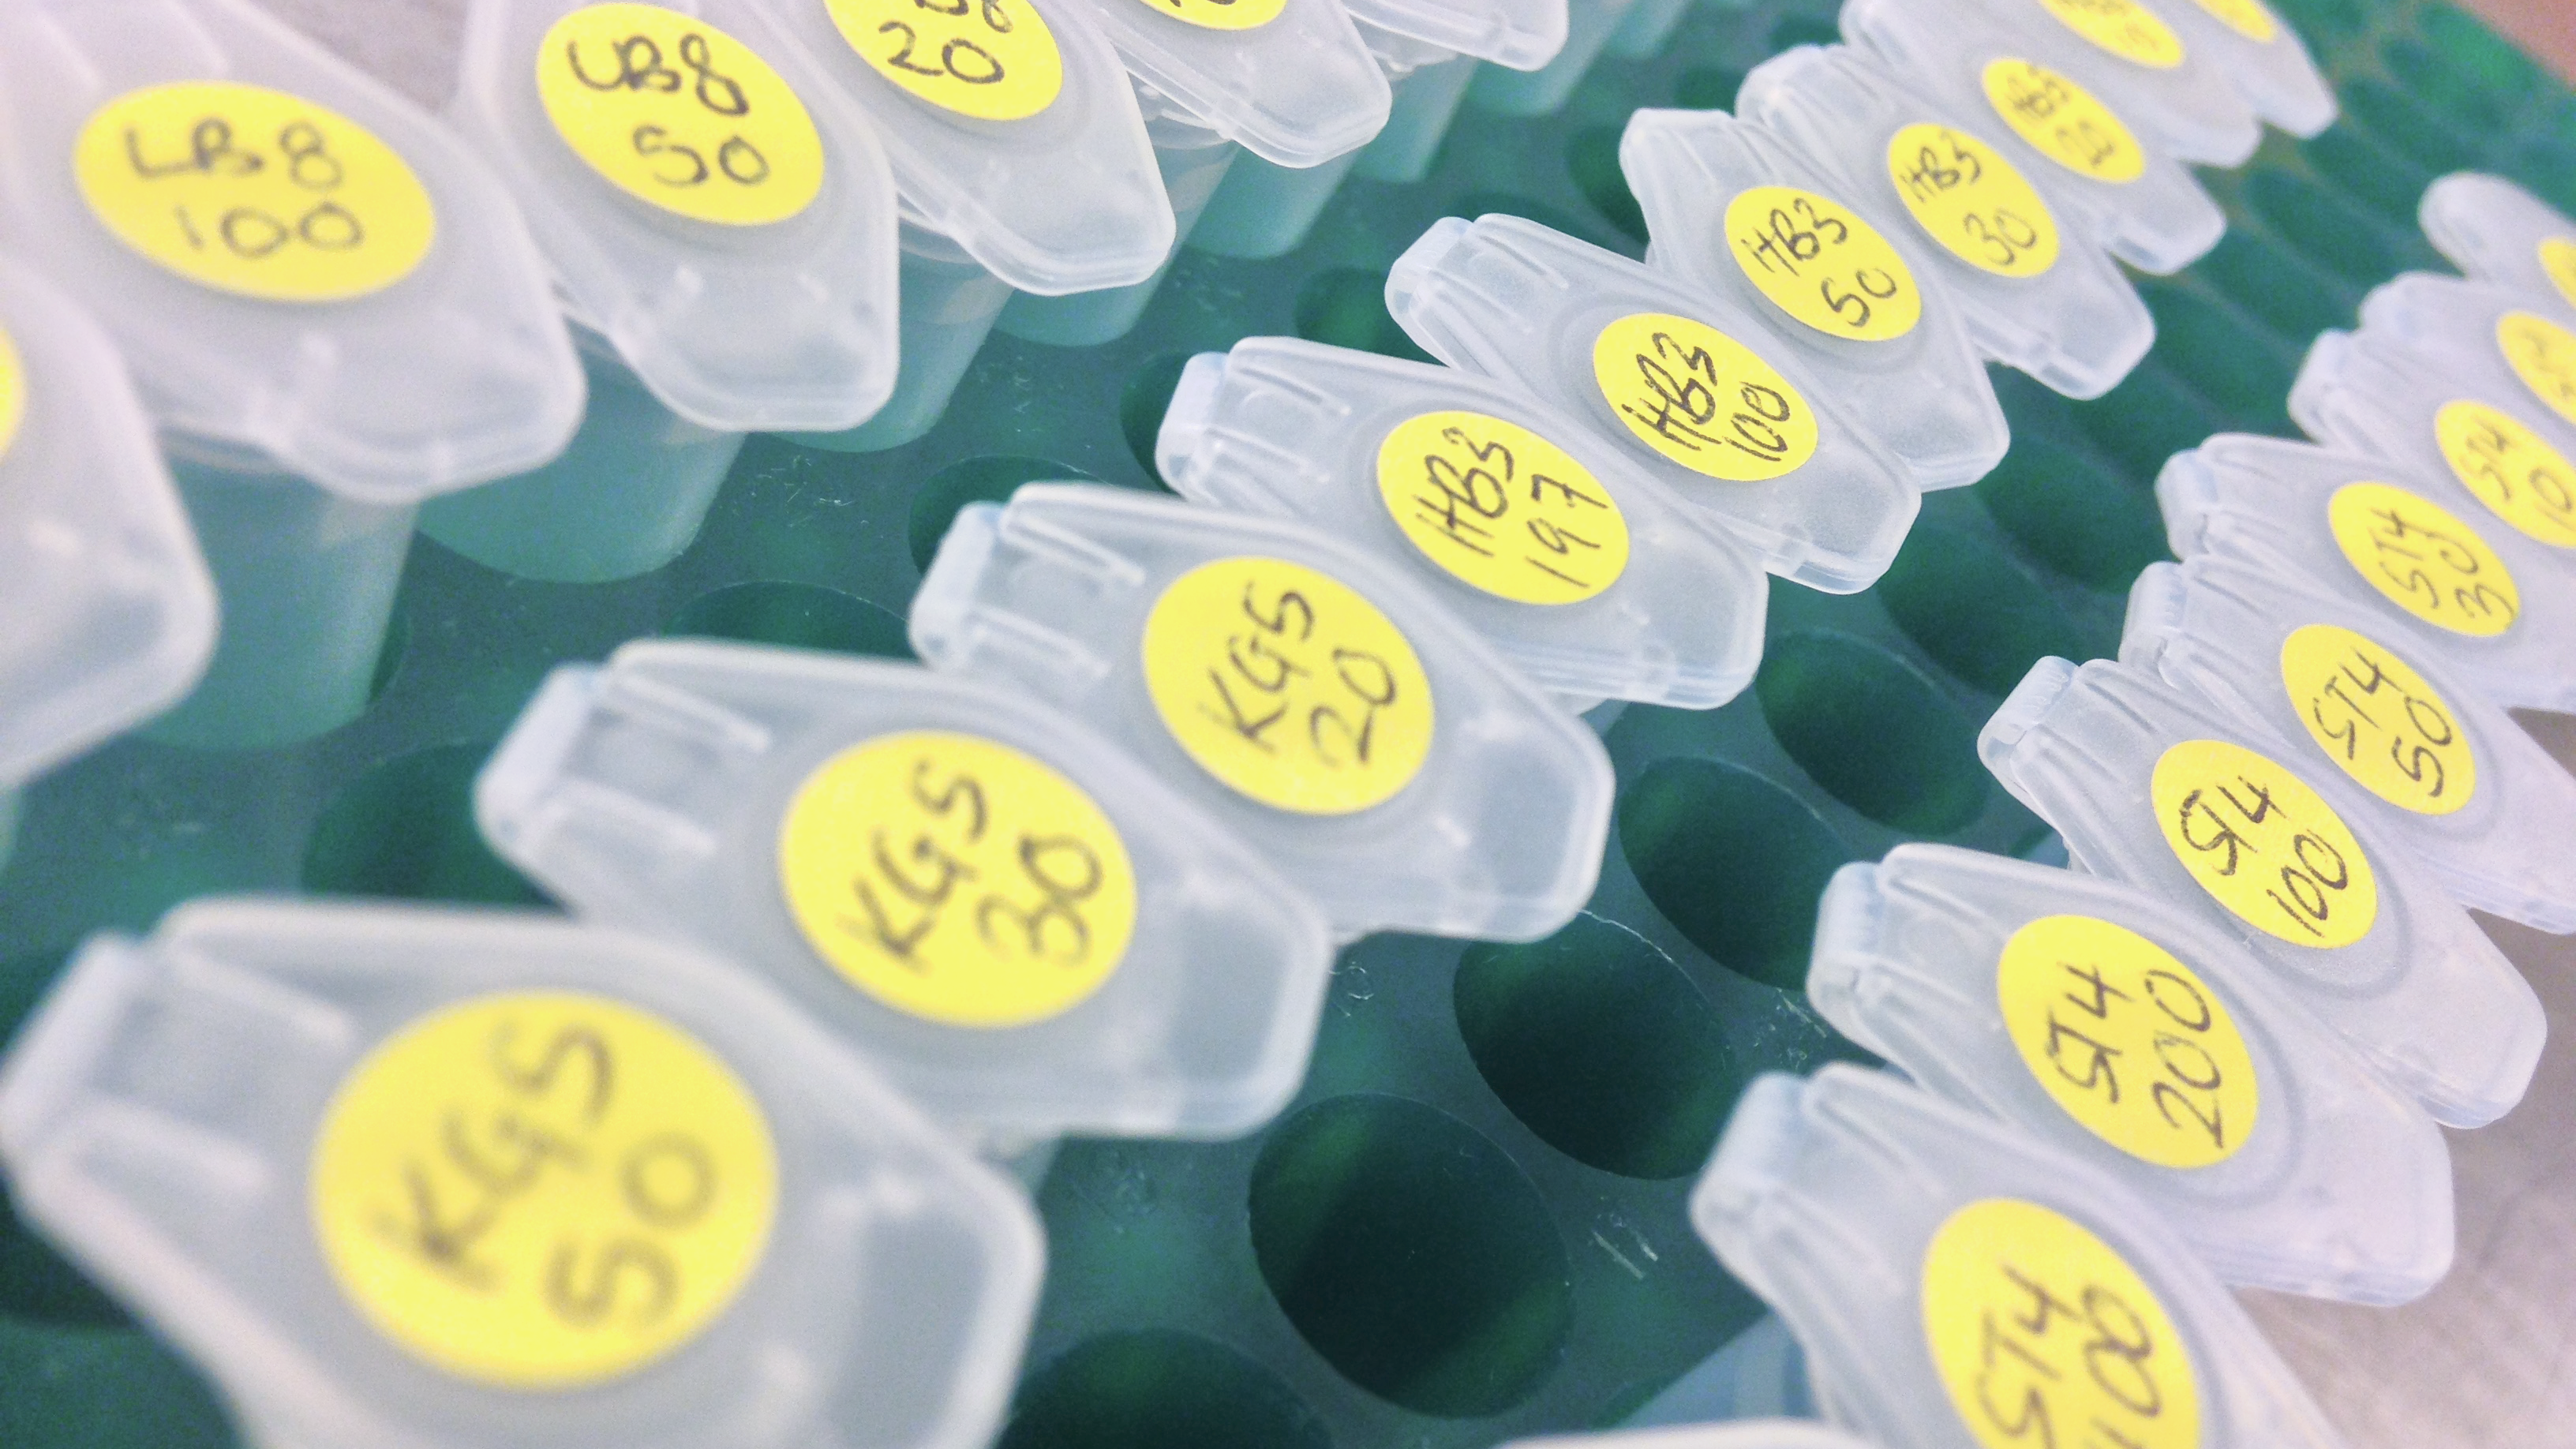
\includegraphics[width=\textwidth]{graphics/pic/20180120_eppendorf_tubes.png}
\end{figure}